\documentclass[a4paper, 14pt]{extarticle}

% Поля
%--------------------------------------
\usepackage{geometry}
\geometry{a4paper,tmargin=2cm,bmargin=2cm,lmargin=3cm,rmargin=1cm}
%--------------------------------------


%Russian-specific packages
%--------------------------------------
\usepackage[T2A]{fontenc}
\usepackage[utf8]{inputenc} 
\usepackage[english, main=russian]{babel}
%--------------------------------------

\usepackage{textcomp}

% Красная строка
%--------------------------------------
\usepackage{indentfirst}               
%--------------------------------------             


%Graphics
%--------------------------------------
\usepackage{graphicx}
\graphicspath{ {./images/} }
\usepackage{wrapfig}
%--------------------------------------

% Полуторный интервал
%--------------------------------------
\linespread{1.3}                    
%--------------------------------------

%Выравнивание и переносы
%--------------------------------------
% Избавляемся от переполнений
\sloppy
% Запрещаем разрыв страницы после первой строки абзаца
\clubpenalty=10000
% Запрещаем разрыв страницы после последней строки абзаца
\widowpenalty=10000
%--------------------------------------

%Списки
\usepackage{enumitem}

%Подписи
\usepackage{caption} 

%Гиперссылки
\usepackage{hyperref}

\hypersetup {
	unicode=true
}

%Рисунки
%--------------------------------------
\DeclareCaptionLabelSeparator*{emdash}{~--- }
\captionsetup[figure]{labelsep=emdash,font=onehalfspacing,position=bottom}
%--------------------------------------

\usepackage{tempora}

%Листинги
%--------------------------------------
\usepackage{listings}
\lstset{
  basicstyle=\ttfamily\footnotesize, 
  %basicstyle=\footnotesize\AnkaCoder,        % the size of the fonts that are used for the code
  breakatwhitespace=false,         % sets if automatic breaks shoulbd only happen at whitespace
  breaklines=true,                 % sets automatic line breaking
  captionpos=t,                    % sets the caption-position to bottom
  inputencoding=utf8,
  frame=single,                    % adds a frame around the code
  keepspaces=true,                 % keeps spaces in text, useful for keeping indentation of code (possibly needs columns=flexible)
  keywordstyle=\bf,       % keyword style
  numbers=left,                    % where to put the line-numbers; possible values are (none, left, right)
  numbersep=5pt,                   % how far the line-numbers are from the code
  xleftmargin=25pt,
  xrightmargin=25pt,
  showspaces=false,                % show spaces everywhere adding particular underscores; it overrides 'showstringspaces'
  showstringspaces=false,          % underline spaces within strings only
  showtabs=false,                  % show tabs within strings adding particular underscores
  stepnumber=1,                    % the step between two line-numbers. If it's 1, each line will be numbered
  tabsize=2,                       % sets default tabsize to 8 spaces
  title=\lstname                   % show the filename of files included with \lstinputlisting; also try caption instead of title
}
%--------------------------------------

%%% Математические пакеты %%%
%--------------------------------------
\usepackage{amsthm,amsfonts,amsmath,amssymb,amscd}  % Математические дополнения от AMS
\usepackage{mathtools}                              % Добавляет окружение multlined
\usepackage[perpage]{footmisc}
%--------------------------------------

%--------------------------------------
%			НАЧАЛО ДОКУМЕНТА
%--------------------------------------

\begin{document}

%--------------------------------------
%			ТИТУЛЬНЫЙ ЛИСТ
%--------------------------------------
\begin{titlepage}
\thispagestyle{empty}
\newpage


%Шапка титульного листа
%--------------------------------------
\vspace*{-60pt}
\hspace{-65pt}
\begin{minipage}{0.3\textwidth}
\hspace*{-20pt}\centering

\includegraphics[width=\textwidth]{emblem}
\end{minipage}
\begin{minipage}{0.67\textwidth}\small \textbf{
\vspace*{-0.7ex}
\hspace*{-6pt}\centerline{Министерство науки и высшего образования Российской Федерации}
\vspace*{-0.7ex}
\centerline{Федеральное государственное бюджетное образовательное учреждение }
\vspace*{-0.7ex}
\centerline{высшего образования}
\vspace*{-0.7ex}
\centerline{<<Московский государственный технический университет}
\vspace*{-0.7ex}
\centerline{имени Н.Э. Баумана}
\vspace*{-0.7ex}
\centerline{(национальный исследовательский университет)>>}
\vspace*{-0.7ex}
\centerline{(МГТУ им. Н.Э. Баумана)}}
\end{minipage}
%--------------------------------------

%Полосы
%--------------------------------------
\vspace{-25pt}
\hspace{-35pt}\rule{\textwidth}{2.3pt}

\vspace*{-20.3pt}
\hspace{-35pt}\rule{\textwidth}{0.4pt}
%--------------------------------------

\vspace{1.5ex}
\hspace{-35pt} \noindent \small ФАКУЛЬТЕТ\hspace{80pt} <<Информатика и системы управления>>

\vspace*{-16pt}
\hspace{47pt}\rule{0.83\textwidth}{0.4pt}

\vspace{0.5ex}
\hspace{-35pt} \noindent \small КАФЕДРА\hspace{50pt} <<Теоретическая информатика и компьютерные технологии>>

\vspace*{-16pt}
\hspace{30pt}\rule{0.866\textwidth}{0.4pt}
  
\vspace{11em}

\begin{center}
\Large {\bf Лабораторная работа № 6.1} \\ 
\large {\bf по курсу <<Компьютерные сети>>} \\
\large <<Разработка FTP-клиента и FTP-сервера>> 
\end{center}\normalsize

\vspace{8em}


\begin{flushright}
  {Студент группы ИУ9-32Б Волохов А. В. \hspace*{15pt}\\ 
  \vspace{2ex}
  Преподаватель Посевин Д. П.\hspace*{15pt}}
\end{flushright}

\bigskip

\vfill
 

\begin{center}
\textsl{Москва 2023}
\end{center}
\end{titlepage}
%--------------------------------------
%		КОНЕЦ ТИТУЛЬНОГО ЛИСТА
%--------------------------------------

\renewcommand{\ttdefault}{pcr}

\setlength{\tabcolsep}{3pt}
\newpage
\setcounter{page}{2}
\section{Задание}\label{Sect::task}
Рассматривается задача разработки FTP-клиента на языке GO на основе
пакета

Задача 1: Реализовать FTP-клиент и запустить его .

Задача 2: Протестировать соединение GO FTP-клиента с установленным на
сервере students.yss.su FTP-сервером со следующими параметрами доступа:
ftp-host: students.yss.su
login: ftpiu8
passwd: 3Ru7yOTA

Задача 3: Реализовать следующие функции:
загрузку файла GO FTP-клиентом на FTP-сервер;
скачивание файла GO FTP-клиентом с FTP-сервера;
создание директории go ftp клиентом на FTP-сервере;
удаление GO FTP-клиентом файла на FTP-сервере;
получение содержимого директории на FTP-сервере с помощью GO FTP-
клиента.

Кроме того, рассматривается задача разработки FTP-сервера на языке GO.

Задача 1: Реализовать FTP-сервер на языке GO.

Задача 2: Протестировать соединение FTP-клиента (для тестирования
можно использовать консольную версию FTP-клиента используемой
операционной системы или FileZilla, WinSCP и д.р.) с реализованным FTP-
сервером. Параметры доступа к ftp серверу могут быть заданы в коде программы
или во внешнем конфигурационном файле.

Задача 3: FTP-сервер должен обладать следующими функциями:
поддерживать авторизацию клиента на FTP-сервере;
передавать клиенту список содержимого заданной директории FTP-
сервера по запросу;
позволять клиенту скачивать файлы из заданной директории FTP сервера
по запросу;◦ позволять клиенту загружать файлы в заданную директорию FTP сервера
по запросу;
позволять клиенту создавать директории на FTP-сервере по запросу;
позволять клиенту удалять директории на FTP-сервере по запросу.

Исходный код программы представлен в листингах~\ref{lst:code1}--~\ref{lst:code2}--~\ref{lst:code3}--~\ref{lst:code4}--~\ref{lst:code5}--~\ref{lst:code6}.

\begin{figure}[!htb]
\begin{lstlisting}[language={Go},caption={client.go},label={lst:code1}]
package main

import (
	"bufio"
	"fmt"
	"github.com/jlaffaye/ftp"
	"io"
	"os"
	"path"
	"strings"
)

const (
	ftpHost  = "students.yss.su"
	ftpLogin = "ftpiu8"
	ftpPass  = "3Ru7yOTA"
)

func main() {
	client, err := ftp.Dial(ftpHost + ":21")
	if err != nil {
		panic(err)
	}
	defer client.Quit()
	err = client.Login(ftpLogin, ftpPass)
	if err != nil {
		panic(err)
	}
	fmt.Println("FTP client connected successfully!")
	scanner := bufio.NewScanner(os.Stdin)
	for {
		fmt.Print("Введите команду (upload, download, create, delete, list, exit): ")
		scanner.Scan()
		command := scanner.Text()

		switch strings.ToLower(command) {
		case "upload":
			fmt.Print("Введите локальный путь к файлу: ")
			scanner.Scan()
			localPath := scanner.Text()
			fmt.Print("Введите удаленный путь для сохранения файла: ")
			scanner.Scan()
			remotePath := scanner.Text()
			uploadFile(client, localPath, remotePath)

		case "download":
			fmt.Print("Введите удаленный путь к файлу: ")
			scanner.Scan()
			remotePath := scanner.Text()
			fmt.Print("Введите локальный путь для сохранения файла: ")
			scanner.Scan()
			localPath := scanner.Text()
			downloadFile(client, remotePath, localPath)
\end{lstlisting}
\end{figure}

\newpage

\begin{figure}[!htb]
\begin{lstlisting}[language={Go},caption={client.go - продолжение},label={lst:code2}]
case "create":
			fmt.Print("Введите имя новой директории: ")
			scanner.Scan()
			directoryName := scanner.Text()
			createDirectory(client, directoryName)

		case "delete":
			fmt.Print("Введите удаленный путь к файлу для удаления: ")
			scanner.Scan()
			remotePath := scanner.Text()
			deleteFile(client, remotePath)

		case "list":
			fmt.Print("Введите удаленный путь: ")
			scanner.Scan()
			remotePath := scanner.Text()
			listDirectory(client, remotePath)

		case "exit":
			fmt.Println("Выход из программы.")
			return

		default:
			fmt.Println("Неверная команда. Пожалуйста, введите корректную команду.")
		}
	}
}

func uploadFile(client *ftp.ServerConn, localPath, remotePath string) {
	file, err := os.Open(localPath)
	if err != nil {
		panic(err)
	}
	defer file.Close()

	err = client.Stor(remotePath+"/"+getFileName(localPath), file)
	if err != nil {
		panic(err)
	}
	fmt.Printf("File %s uploaded successfully.\n", localPath)
}


\end{lstlisting}
\end{figure}

\newpage
\begin{figure}[!htb]
\begin{lstlisting}[language={Go},caption={client.go - продолжение},label={lst:code3}]
func downloadFile(client *ftp.ServerConn, remotePath, localPath string) {
	resp, err := client.Retr(remotePath)
	if err != nil {
		panic(err)
	}
	defer resp.Close()

	file, err := os.Create(localPath + "/" + getFileName(remotePath))
	if err != nil {
		panic(err)
	}
	defer file.Close()

	_, err = io.Copy(file, resp)
	if err != nil {
		panic(err)
	}

	fmt.Printf("File %s downloaded successfully.\n", remotePath)
}

func createDirectory(client *ftp.ServerConn, directoryName string) {
	err := client.MakeDir(directoryName)
	if err != nil {
		panic(err)
	}
	fmt.Printf("Directory %s created successfully.\n", directoryName)
}

func deleteFile(client *ftp.ServerConn, remotePath string) {
	err := client.Delete(remotePath)
	if err != nil {
		panic(err)
	}
	fmt.Printf("File %s deleted successfully.\n", remotePath)
}

func listDirectory(client *ftp.ServerConn, directoryPath string) {
	entries, err := client.List(directoryPath)
	if err != nil {
		panic(err)
	}
	fmt.Printf("Directory listing for %s:\n", directoryPath)
	for _, entry := range entries {
		fmt.Println(entry.Name)
	}
}

func getFileName(filePath string) string {
	_, file := path.Split(filePath)
	return file
}
\end{lstlisting}
\end{figure}

\newpage
\begin{figure}[!htb]
\begin{lstlisting}[language={Go},caption={server.go},label={lst:code3}]
package main

import (
	"flag"
	filedriver "github.com/goftp/file-driver"
	"github.com/goftp/server"
	"log"
)

func main() {
	var (
		root = flag.String("root", "/home/alexandr/BMSTU_git/IU9-CN-GO/lab6.1/server/server_space", "Root directory to serve")
		user = flag.String("user", "Sasha", "Username for login")
		pass = flag.String("pass", "123", "Password for login")
		port = flag.Int("port", 2121, "Port")
		host = flag.String("host", "", "Host")
	)
	flag.Parse()
	if *root == "" {
		log.Fatalf("Please set a root to serve with -root")
	}

	factory := &filedriver.FileDriverFactory{
		RootPath: *root,
		Perm:     server.NewSimplePerm("user", "group"),
	}

	opts := &server.ServerOpts{
		Factory:  factory,
		Port:     *port,
		Hostname: *host,
		Auth:     &server.SimpleAuth{Name: *user, Password: *pass},
	}

	log.Printf("Starting ftp server on %v:%v", opts.Hostname, opts.Port)
	log.Printf("Username %v, Password %v", *user, *pass)
	server := server.NewServer(opts)
	err := server.ListenAndServe()
	if err != nil {
		log.Fatal("Error starting server:", err)
	}
}

\end{lstlisting}
\end{figure}

\newpage

\begin{figure}[!htb]
	\centering
	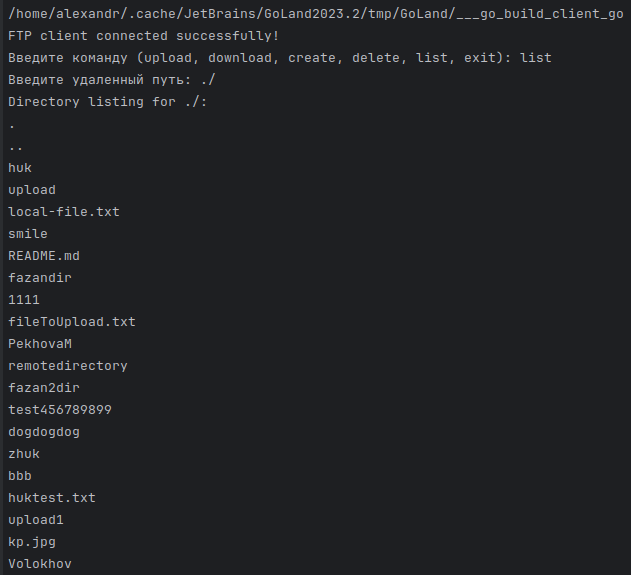
\includegraphics[width=0.8\textwidth]{res1.png}
\caption{Клиент}
\label{fig:img1}
\end{figure}

\begin{figure}[!htb]
	\centering
	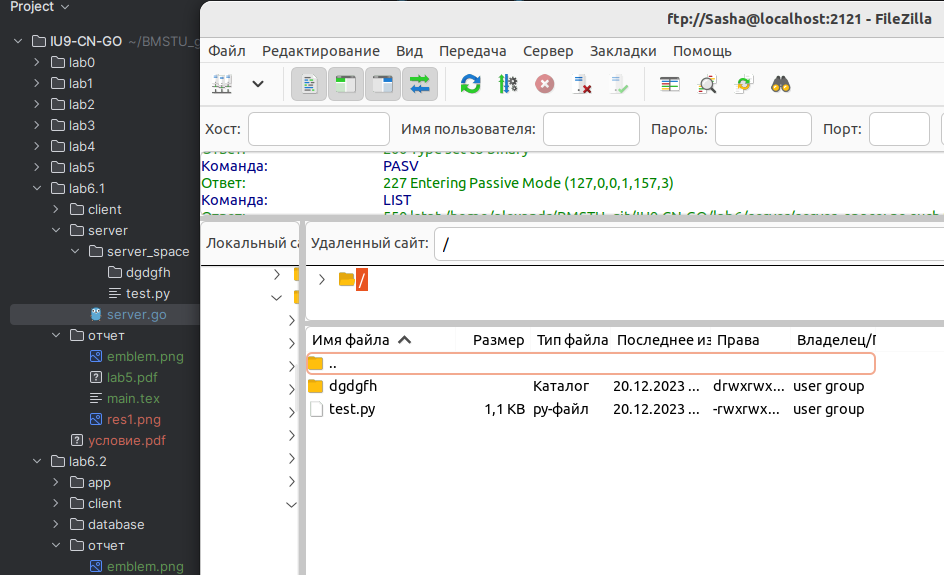
\includegraphics[width=0.8\textwidth]{res2.png}
\caption{Сервер}
\label{fig:img2}
\end{figure}





\end{document}
